% Teorema Órbita-Estabilizador
% Compilar con: pdflatex orbit_stabilizer.tex
\documentclass[tikz,border=10pt]{standalone}
\usepackage{tikz}
\usepackage{amsmath,amssymb}
\usepackage{xcolor}
\definecolor{gdlblue}{RGB}{41, 98, 168}
\definecolor{gdlred}{RGB}{191, 49, 49}
\definecolor{gdlgreen}{RGB}{30, 130, 76}
\definecolor{gdlorange}{RGB}{217, 130, 30}
\definecolor{gdlpurple}{RGB}{118, 56, 138}
\definecolor{gdlgray}{RGB}{140, 140, 140}
\definecolor{gdlyellow}{RGB}{190, 140, 10}
\usetikzlibrary{arrows.meta, positioning, shapes.geometric, calc}

\begin{document}
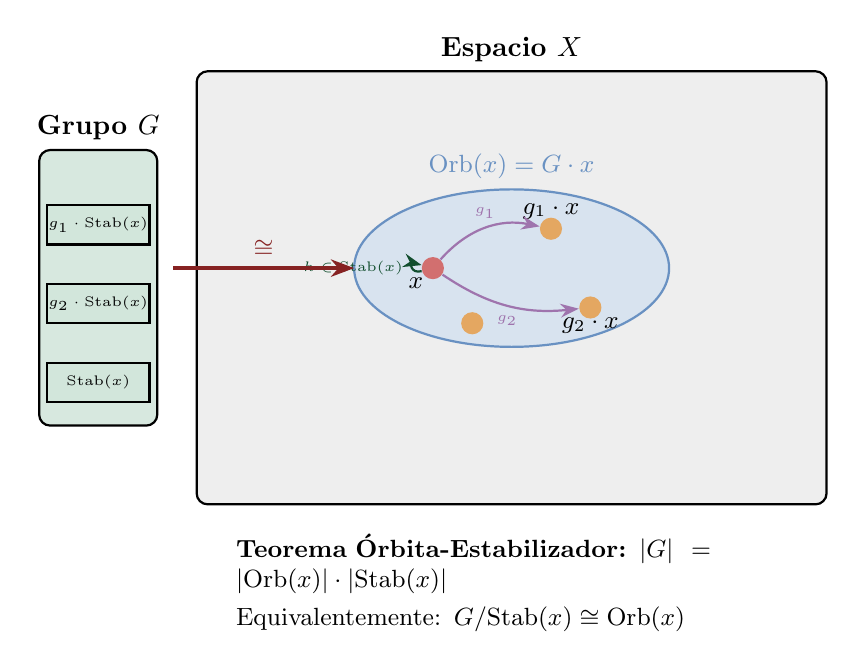
\begin{tikzpicture}[
    >=Stealth,
    point/.style={circle, fill=#1, minimum size=8pt, inner sep=0pt},
    orbit/.style={ellipse, draw=gdlblue!70, thick, minimum width=4cm, minimum height=2cm}
]

% Espacio X
\draw[thick, fill=gdlgray!15, rounded corners] (-3,-2.5) rectangle (5,3);
\node[above] at (1, 3) {\textbf{Espacio $X$}};

% Órbita de x
\node[orbit, fill=gdlblue!18] (orb) at (1, 0.5) {};
\node[above, gdlblue!70, font=\small] at (orb.north) {$\mathrm{Orb}(x) = G \cdot x$};

% Puntos en la órbita
\node[point=gdlred!70] (x) at (0, 0.5) {};
\node[below left, font=\small] at (x) {$x$};

\node[point=gdlorange!70] (gx1) at (1.5, 1) {};
\node[above, font=\small] at (gx1) {$g_1 \cdot x$};

\node[point=gdlorange!70] (gx2) at (2, 0) {};
\node[below, font=\small] at (gx2) {$g_2 \cdot x$};

\node[point=gdlorange!70] (gx3) at (0.5, -0.2) {};

% Flechas de acción
\draw[->, thick, gdlpurple!70] (x) to[bend left=30] node[above, font=\tiny] {$g_1$} (gx1);
\draw[->, thick, gdlpurple!70] (x) to[bend right=20] node[below, font=\tiny] {$g_2$} (gx2);

% Estabilizador (flechas que vuelven a x)
\draw[->, thick, gdlgreen!60!black, loop left, looseness=5] (x) to node[left, font=\tiny] {$h \in \mathrm{Stab}(x)$} (x);

% Grupo G
\draw[thick, fill=gdlgreen!18, rounded corners] (-5,-1.5) rectangle (-3.5,2);
\node[above] at (-4.25, 2) {\textbf{Grupo $G$}};

% Cosets de Stab(x)
\foreach \y/\label in {1.3/$g_1 \cdot \mathrm{Stab}(x)$, 0.3/$g_2 \cdot \mathrm{Stab}(x)$, -0.7/$\mathrm{Stab}(x)$} {
    \draw[thick, fill=gdlgreen!20] (-4.9, \y) rectangle (-3.6, \y-0.5);
    \node[font=\tiny] at (-4.25, \y-0.25) {\label};
}

% Flecha de biyección
\draw[->, very thick, gdlred!70!black] (-3.3, 0.5) -- node[above, font=\small] {$\cong$} (-1, 0.5);

% Teorema
\node[font=\small, text width=7cm] at (1, -3.5) {
    \textbf{Teorema Órbita-Estabilizador:}
    $|G| = |\mathrm{Orb}(x)| \cdot |\mathrm{Stab}(x)|$\\[0.3em]
    Equivalentemente: $G/\mathrm{Stab}(x) \cong \mathrm{Orb}(x)$
};

\end{tikzpicture}
\end{document}
